\documentclass[dvipdfmx]{beamer}

\usepackage{graphics}
\usepackage{amsmath}
\usepackage{amssymb}
\usepackage{ascmac}
\usepackage{txfonts}
\usepackage{bm}
\usepackage{docmute}
\usepackage{tikz}
\usetikzlibrary{calc}
\usetikzlibrary{intersections}

\usetheme{Madrid}
\usefonttheme{professionalfonts}


\title{5月第1課題}
\author{近藤 綜太}

\begin{document}
	\maketitle
	\begin{frame}{はじめに}
		緊急事態宣言が延長され,休校期間が伸びそうになってきました.
		そこで,学校がなくとも学習の進度を守れるようにここで
		いくつかの課題を出していきたいと思います.

		発展的な問題を出すこともあるので,
		グループのみんなで相談しながら解いてください.
	\end{frame}

	\begin{frame}{問題1}
		図の四角形 $\mathrm{ABCD}$は平行四辺形である.
		この平行四辺形の面積を二等分する直線のうち,
		傾きが1であるものを求めよ.
		\begin{figure}[htbp]
			\centering
			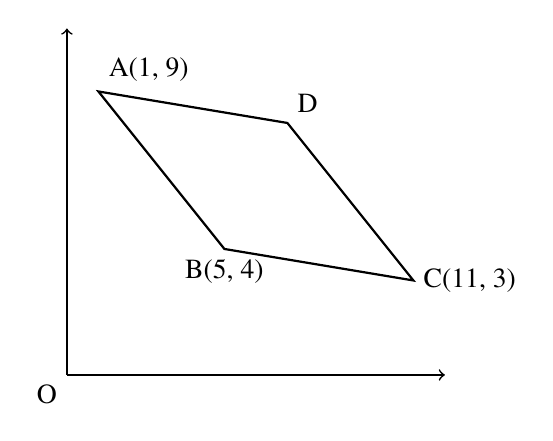
\begin{tikzpicture}[scale = 0.4]
				\draw[semithick, ->] (0, 0)node[below left]{O}--(12, 0);
				\draw[semithick, ->] (0, 0)--(0, 11);

				\coordinate[](a) at (1, 9);
				\coordinate[](b) at (5, 4);
				\coordinate[](c) at (11, 3);
				\coordinate[](d) at (7, 8);

				\draw[thick] (a)node[above right]{A(1, 9)}--(b)node[below]{B(5, 4)}--(c)node[right]{C(11, 3)}--(d)node[above right]{D}--cycle;
			\end{tikzpicture}
			\caption{平行四辺形}
		\end{figure}
	\end{frame}

	\begin{frame}{問題2}
		\begin{columns}
			\begin{column}{0.5\textwidth}\centering
				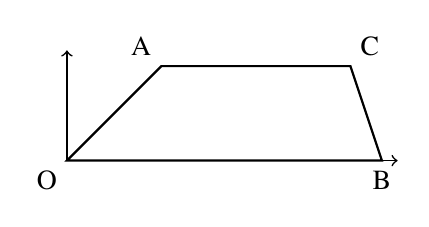
\begin{tikzpicture}[scale = 0.2]
					\draw[semithick, ->] (0, 0)node[below left]{O}--(21, 0);
					\draw[semithick, ->] (0, 0)--(0, 7);

					\coordinate[](a) at (6, 6);
					\coordinate[](b) at (20, 0);
					\coordinate[](c) at (18, 6);
					\draw[thick] (a)node[above left]{A}--(c)node[above right]{C}--(b)node[below]{B}--(0, 0)--cycle;
				\end{tikzpicture}

				\begin{gather*}
					\mathrm{A}:(6, 6)\\
					\mathrm{B}:(20, 0)\\
					\mathrm{C}:(18, 6)
				\end{gather*}
			\end{column}

			\begin{column}{0.5\textwidth}
				以下の条件を満たす直線をそれぞれ求めよ.
				\begin{enumerate}
					\item 点Aを通り,台形AOBCの面積を二等分にする直線
					\item 点(12, 6)を通り,台形AOBCの面積を二等分にする直線
					\item 傾き1で,台形AOBCの面積を二等分にする直線
				\end{enumerate}
			\end{column}

		\end{columns}
	\end{frame}
\end{document}
